\documentclass[sigconf,nonacm]{acmart}
\pdfpagewidth=8.27in
\pdfpageheight=11.7in

\usepackage{pgfplots}
%\usepgfplotslibrary{external}
\pgfplotsset{width=6.5cm,compat=1.15}
\pgfplotsset{every axis legend/.append style={at={(0.01, 0.99)},anchor=north west,},every node near coord/.append style={font=\small}}
\pgfplotsset{scale=0.8}
\usepackage{subcaption}
\usepackage{minted}
\usepackage{booktabs}

\begin{document}

\title{An analysis of the performance of Graph Nets when used to execute graph algorithms.}

\author{Oliver Hope $\langle$oh260$\rangle$}
\affiliation{\institution{Jesus College}}

\renewcommand{\shortauthors}{O. Hope}

\maketitle

\section{Introduction}

Graph neural networks (GNNs) have been researched for quite a while with the first paper on them being written in 2004\cite{first-gnn}. More recently there has been an increased interest in the use of GNNs in different areas of deep learning. This is due to how they easily allow researchers to specify certain structure and relations to their data representation to help guide the learning process and increase generalisability of solutions.

Given this interest, DeepMind introduced a new library called Graph Nets\cite{graph-nets} which implements a framework for easily creating GNNs on top of TensorFlow\cite{tensorflow}. This is to reduce development time while allowing models to benefit from all the optimisations of executing tensor transformations and learning algorithms that TensorFlow brings.

TensorFlow is a library designed primarily for machine learning uses. However, to achieve this it builds on top of a dataflow paradigm where computations are represented as directed acyclic graphs (DAGs). This means it is possible to use it for generic dataflow programming as long as you are happy to work with tensors and tensor operations for your dataflow.

In the same vein, although Graph Nets itself is designed for executing GNNs for machine learning, it is possible to use the abstraction to execute generic graph algorithms. This paper examines the latter statement. It seeks to use Graph Nets atop TensorFlow to execute generic graph algorithms without any machine learning aspect. This is useful for two reasons. The first reason is that if it does perform well then it shows that maybe this is a worthwhile area of graph processing to examine and a viable method for executing graph algorithms. The second reason is that machine learning takes a long time to train and it would be interesting to see if the GNN framework has an impact on this (i.e. training times could be reduced with a different implementation of the abstraction).

To assess the findings from the experiments run in this paper, there will be a comparison against GraphChi\cite{graphchi} running the same experiments. The reasons for choosing this framework are its high performance when running on a single node which is how we will be running Graph Nets.

\section{Theory}

Before delving into the algorithms run and the graph execution, we will explain the abstractions used by both frameworks for performing graph computations.

\subsection{Graph Nets abstraction}\label{section:abstraction}

The basic structure of a graph computation used in Graph Nets is a GN block which takes a graph as input and returns a graph as output. Computation in a graph block proceeds in three stages which can all be customised (and generally rely on parameters which can bet trained). These three stages are illustrated in figure~\ref{fig:graph-nets-stages}.

\begin{figure}[H]
    \centering
    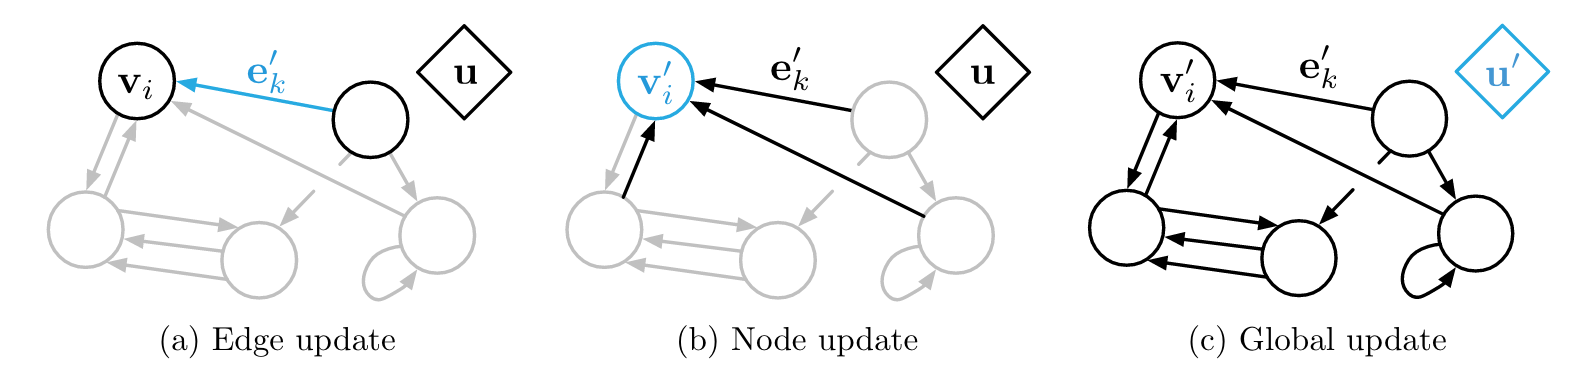
\includegraphics[width=0.5\textwidth]{graph-nets-stages.png}
    \caption{Stages in a Graph Nets GN block used in computation.}
    \label{fig:graph-nets-stages}
\end{figure}

The first stage is an Edge Block. In the Edge Block we are able to update the value of each edge using the value of its source and destination values, its previous value and any global values.

The second stage is a Node Block. In the Node Block we can update the value of a node using its previous value and any global values. We can also use the values of any incoming and outgoing edgers. However, this is not as straightforward as in other frameworks because we only get given a single value. This value has been created from a reducer function over all the edges presented (and can be customised, but can still only return a single value).

The final stage is a Global Block. This takes as input the current global values and a reducer run over all the node values and reduced edge values input in the previous stage. This returns the newly updated global values.

A visualisation of all of these stages put together can be seen in figure~\ref{fig:graph-nets-block}.

\begin{figure}[H]
    \centering
    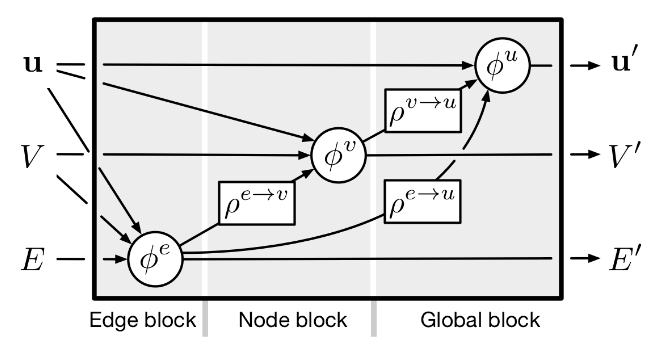
\includegraphics[width=0.4\textwidth]{graph-nets-full.png}
    \caption{Full GN Block}
    \label{fig:graph-nets-block}
\end{figure}

\subsection{GraphChi abstraction}

GraphChi takes quite a different approach. This is because it was designed as a high performance generic graph processing framework to be run on a single machine with not distributed processing capability. It takes some cues from the bulk synchronous parallel model for graph processing first popularised by Pregel\cite{pregel} however is makes a few changes. The first of these is that it moves to the asynchronous model used by many later systems where updates can use the latest values available rather than every vertex executing in lockstep. Also, to get around the issues of small memory on a single machine, GraphChi adopts a method to chop a graph into smaller parts and then uses a new parallel sliding window method to process these shards. There are further extensions added to the solution proposed that allow for the graph to be modified by a computation.

 We will not go into further detail on GraphChi as it is simply being used as a comparison during the benchmarking process (the reason fro this choice being its aim to be fast and efficient on a single system).

\subsection{Algorithm implementation}

From section~\ref{section:abstraction} we can see that Graph Nets uses a system not unlike the bulk synchronous parallel (BSP) model of Pregel with supersteps of graph computation. In fact, the only real difference is the extra constraints. Those constraints are that all values must be elements of tensors and that message passing is complicated by the fact that values of incoming edges must be reduced before a node can see them. This makes more complicated algorithms harder to implement.

The algorithms used for testing in this study have been connected components (CC) single source shortest path (SSSP) and page rank (PR). This is because they allow for testing different aspects of performance of a framework. PR allows us to test how the system is impacted by calculations during steps whereas the other two methods examine how well the message passing itself works as the number of steps is not fixed (with SSSP examining if it can take advantage of most of the graph not experiencing work and CC examining general propagation across the whole graph).

Graph algorithms of these types can be implemented in a BSP style by using only an edge and node block and relying the sources when updating edge values and only the incoming edges when updating node values.

\subsubsection{Edge Block}

The edge block is created as shown in listing~\ref{listing:edge-block}. It is a fairly straightforward for simple algorithms such as CC. We implement it by choosing which features we require to calculate the new edge values (in this example just the previous value and the sender nodes). Then we give it a sonnet module implementing the model to perform the calculation. This is shown in the class \texttt{CCEdge}. The important code here is in the build function which takes all the inputs as a tensor and outputs all the new edge values as a tensor. In this example the edges hold their length and a message and after this is concatenated the source node value. Therefore we return the 1st and 2nd elements, which retains the edge length first and replaces the previous message with the source value.

\begin{listing}[ht]
\small{}
%%TC:ignore
\begin{minted}{python}
class CCEdge(snt.AbstractModule):
  def __init__(self, name="ccedge"):
    super(CCEdge, self).__init__(name=name)

  def _build(self, inputs):
    return tf.stack([inputs[:,0], inputs[:,2]], 1)
                          
cc_edge_block = lambda: blocks.EdgeBlock(
    edge_model_fn=lambda: CCEdge(output_size=10),
    use_edges=True,
    use_receiver_nodes=False,
    use_sender_nodes=True,
    use_globals=False,
    name="edge_block")
\end{minted}
%%TC:endignore
\caption{The code to create an Edge Block for the connected components algorithm.}
\label{listing:edge-block}
\end{listing}

\subsubsection{Node Block}

The node block implementation for CC can be seen in listing~\ref{listing:node-block}. We can see this is very similar to the edge block. However, this time we must specify a \texttt{received\_edges\_reducer} which for CC we use the minimum as we wish to propagate the minimum node id in each component. The node model module is slightly more complicated as there is more logic involved. Here we represent each node by its component id and whether it votes to halt (important later). As set when creating the node block, the input are the reduced edge values concatenated onto the previous node values. For CC we want the result to be the minimum id seen along any edge and so this is what the calculation finds. Finally, we set if we should halt depending on if the node's value was actually updated in this step or not.

\begin{listing}[ht]
\small{}
%%TC:ignore
\begin{minted}{python}
class CCNode(snt.AbstractModule):
  def __init__(self, name="ccnode"):
    super(CCNode, self).__init__(name=name)

  def _build(self, inputs):
    minimums = tf.math.minimum(inputs[:,1], inputs[:,2])
    changed = tf.dtypes.cast(
                tf.math.equal(
                  minimums, inputs[:,2]), dtype=tf.float32)
    return tf.stack([minimums, changed], 1)
                          
cc_node_block = lambda: blocks.NodeBlock(
    node_model_fn=lambda: CCNode(),
    use_received_edges=True,
    use_sent_edges=False,
    use_nodes=True,
    use_globals=False,
    received_edges_reducer=tf.math.unsorted_segment_min,
    name="node_block"
\end{minted}
%%TC:endignore
\caption{The code to create a Node Block for the connected components algorithm.}
\label{listing:node-block}
\end{listing}

\subsubsection{Algorithm execution}

Finally, when actually executing graph algorithms we often have to perform many iterations and we often do not know how many will be needed in advance. Fortunately, TensorFlow supports while loops in its dataflow. Therefore we can put an entire execution step, built from the blocks described above in the body of a while loop. Then the stopping condition can be a boolean test on whether all nodes have set their vote to halt values. The code used to perform this operation can be seen in listing~\ref{listing:loops}.

\begin{listing}[ht]
\small{}
%%TC:ignore
\begin{minted}{python}
 g0 = input_graphs
 i0 = tf.constant(0)
 # break condition
 c = lambda g, i: tf.equal(
         tf.math.reduce_min(g.nodes[:,1]), 0)
 # loop body
 b = lambda g, i: (sssp_step(g), i+1)
 r = tf.while_loop(c, b, [g0, i0])
\end{minted}
%%TC:endignore
\caption{The code used to loop, running the supersteps until the computation completes}
\label{listing:loops}
\end{listing}

\section{Test Methodology}

The platform used to run all of the experiments was a single virtual machine running in Google Cloud. The particular model being: \texttt{n1-standard-4 (4 vCPUs, 15 GB memory)} running Debian 10.2. The reason to use a single machine was that even though TensorFlow can be run in a distributed manner, that is not designed for this kind of application. Also, the distribution or the execution graph across multiple devices is quite a manual process requiring a lot of tweaking and is outside the scope of this study.

The Graph Nets execution system was tested using three different algorithms on graphs of different scales generated with different methods. GraphChi was also run on all the same graphs with the same algorithms to get a good performance comparison. The algorithms chosen for testing as mentioned above were CC, SSSP and PR. All the Graph Nets implementations were written by the author along with the GraphChi SSSP implementation. The other GraphChi implementations were written by the GraphChi author.

The graphs chosen to run these algorithms were all generated in three separate sets. First of all, random graphs were generated with $10^n$ nodes and $10^{n+1}$ edges for values of $n$ between 1 and 6. The second set was of fully connected graphs with $10^n$ nodes for values of $n$ between 1 and 4 and the third set was of a linear graph with $10^n$ nodes for values of $n$ between 1 and 7. (Final sizes were chosen based on when Graph Nets ran out of memory). The reason for different types of graph was to test how the systems performed for different aspects of worst and average case performance.

\section{Analysis of results}

The results of all the tests can be seen in figures \ref{fig:random}, \ref{fig:fully} and \ref{fig:linear}. We can see that in general, as expected the performance of Graph Nets based execution is on the order of ten to one hundred times slower for most cases. We can also see the GraphChi implementations are always faster for the algorithms used. The graphs show values averaged across all three runs of each test. Error bars are not shown as they were too small to be visible on the scale of the graphs.

% All data input manually inline. Not sure why I did this to myself.
\begin{figure*}
\begin{subfigure}{.3\textwidth}
  \centering
  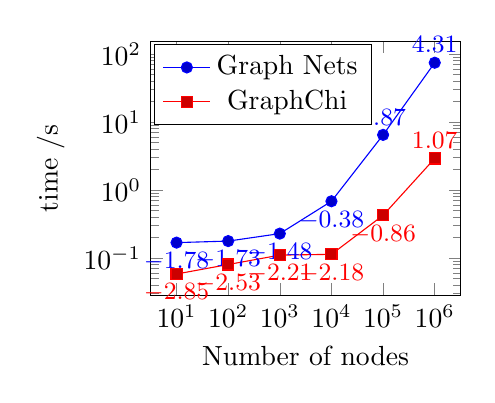
\begin{tikzpicture}
% CC axis
\begin{axis}[
  %ybar,
  ylabel={time /s},
  ymode=log,
  xlabel=Number of nodes,
  symbolic x coords={$10^1$, $10^2$, $10^3$, $10^4$, $10^5$, $10^6$},
  xtick=data,
  nodes near coords,
  nodes near coords align={vertical}
]
\addplot coordinates {
($10^1$,0.168)
($10^2$,0.177)
($10^3$,0.228)
($10^4$,0.683)
($10^5$,6.478)
($10^6$,74.737)
};
\addplot coordinates {
($10^1$,0.058)
($10^2$,0.080)
($10^3$,0.110)
($10^4$,0.113)
($10^5$,0.424)
($10^6$,2.916)
};
    \legend{Graph Nets, GraphChi}
\end{axis}
\end{tikzpicture}
  \caption{CC}
\end{subfigure}%
\begin{subfigure}{.3\textwidth}
  \centering
  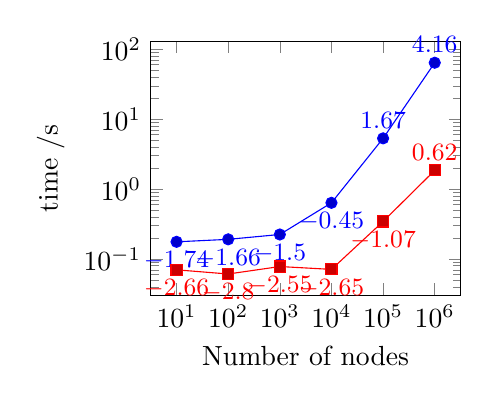
\begin{tikzpicture}
% SSSP axis
\begin{axis}[
  %ybar,
  ymode=log,
  ylabel={time /s},
  xlabel=Number of nodes,
  symbolic x coords={$10^1$, $10^2$, $10^3$, $10^4$, $10^5$, $10^6$},
  xtick=data,
  nodes near coords,
  nodes near coords align={vertical}
]
\addplot coordinates {
($10^1$,0.176)
($10^2$,0.191)
($10^3$,0.224)
($10^4$,0.636)
($10^5$,5.311)
($10^6$,64.110)
};
\addplot coordinates {
($10^1$,0.070)
($10^2$,0.061)
($10^3$,0.078)
($10^4$,0.071)
($10^5$,0.344)
($10^6$,1.852)
};
\legend{};
\end{axis}
\end{tikzpicture}
  \caption{SSSP}
\end{subfigure}
\begin{subfigure}{.3\textwidth}
  \centering
  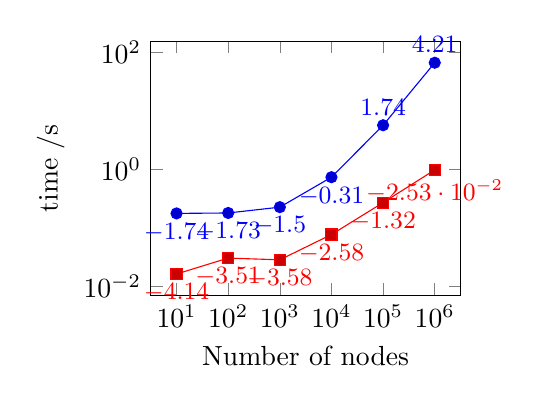
\begin{tikzpicture}
% PR axis
\begin{axis}[
  %ybar,
  ylabel={time /s},
  ymode=log,
  xlabel=Number of nodes,
  symbolic x coords={$10^1$, $10^2$, $10^3$, $10^4$, $10^5$, $10^6$},
  xtick=data,
  nodes near coords,
  nodes near coords align={vertical}
]
\addplot coordinates {
($10^1$,0.175)
($10^2$,0.178)
($10^3$,0.224)
($10^4$,0.731)
($10^5$,5.684)
($10^6$,67.129)
};
\addplot coordinates {
($10^1$,0.016)
($10^2$,0.030)
($10^3$,0.028)
($10^4$,0.076)
($10^5$,0.268)
($10^6$,0.975)
};
\legend{};
\end{axis}
\end{tikzpicture}
  \caption{PR}
\end{subfigure}
\caption{Algorithm execution times running on randomly generated graphs}
\label{fig:random}
\end{figure*}

For the randomly generated graphs we can see that both systems seem to have a doubly exponential increase in the number of nodes contained in the graph. Interestingly, both systems seem to have the same scaling (albeit at different orders of magnitude). This is likely because for these graphs the number of steps needed for completion were similar to the 10 PageRank iterations and updates across the whole graph meant the asynchronicity of GraphChi was not beneficial compared to the synchronous steps in Graph Nets.

\begin{figure*}
\begin{subfigure}{.3\textwidth}
  \centering
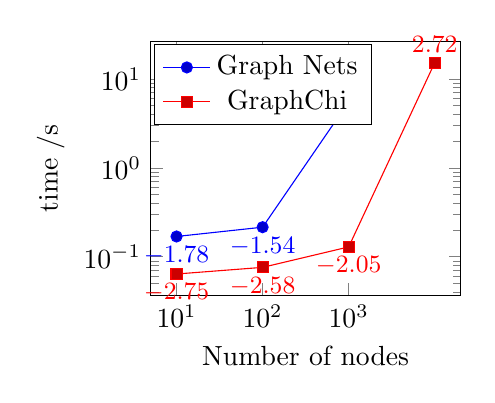
\begin{tikzpicture}
% CCf axis
\begin{axis}[
  %ybar,
  ylabel={time /s},
  ymode=log,
  xlabel=Number of nodes,
  symbolic x coords={$10^1$, $10^2$, $10^3$, $10^4$},
  xtick=data,
  nodes near coords,
  nodes near coords align={vertical}
]
\addplot coordinates {
($10^1$,0.169)
($10^2$,0.215)
($10^3$,5.512)
($10^4$,inf)
};
\addplot coordinates {
($10^1$,0.064)
($10^2$,0.076)
($10^3$,0.129)
($10^4$,15.178)
};
    \legend{Graph Nets, GraphChi}
\end{axis}
\end{tikzpicture}
  \caption{CC}
\end{subfigure}%
\begin{subfigure}{.3\textwidth}
  \centering
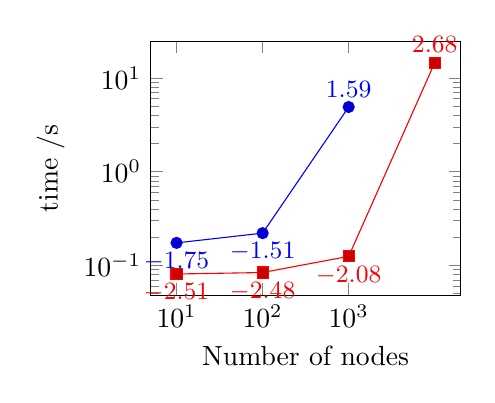
\begin{tikzpicture}
% SSSPf axis
\begin{axis}[
  %ybar,
  ylabel={time /s},
  ymode=log,
  xlabel=Number of nodes,
  symbolic x coords={$10^1$, $10^2$, $10^3$, $10^4$},
  xtick=data,
  nodes near coords,
  nodes near coords align={vertical}
]
\addplot coordinates {
($10^1$,0.174)
($10^2$,0.221)
($10^3$,4.902)
($10^4$,inf)
};
\addplot coordinates {
($10^1$,0.081)
($10^2$,0.084)
($10^3$,0.125)
($10^4$,14.540)
};
    \legend{}
\end{axis}
\end{tikzpicture}
  \caption{SSSP}
\end{subfigure}
\begin{subfigure}{.3\textwidth}
  \centering
  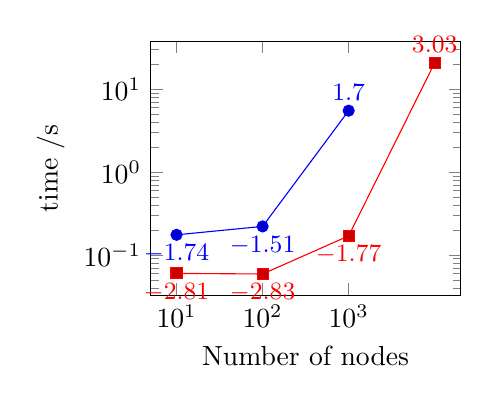
\begin{tikzpicture}
% PRf axis
\begin{axis}[
  %ybar,
  ylabel={time /s},
  ymode=log,
  xlabel=Number of nodes,
  symbolic x coords={$10^1$, $10^2$, $10^3$, $10^4$},
  xtick=data,
  nodes near coords,
  nodes near coords align={vertical}
]
\addplot coordinates {
($10^1$,0.175)
($10^2$,0.221)
($10^3$,5.484)
($10^4$,inf)
};
\addplot coordinates {
($10^1$,0.060)
($10^2$,0.059)
($10^3$,0.170)
($10^4$,20.742)
};
    \legend{}
\end{axis}
\end{tikzpicture}
  \caption{PR}
\end{subfigure}
\caption{Algorithm execution times running on fully connected graphs.}
\label{fig:fully}
\end{figure*}

The results for the fully connected graphs tell a similar story to the random graphs. Both algorithms experience doubly exponential increase of runtime with GraphChi again performing an order of magnitude better than Graph Nets. However one big difference in this example was memory impact. We can see that the series end early for Graph Nets. This was due to out of memory errors. Graph Chi did not share the same problem. The reason for this difference is Graph Nets uses TensorFlow and so expects all of the data to be kept in memory at all times. However as Graph Chi is designed for large graphs it intelligently moves data between memory and disk allowing it to cope with far higher numbers of edges.

\begin{figure*}
\begin{subfigure}{.3\textwidth}
  \centering
  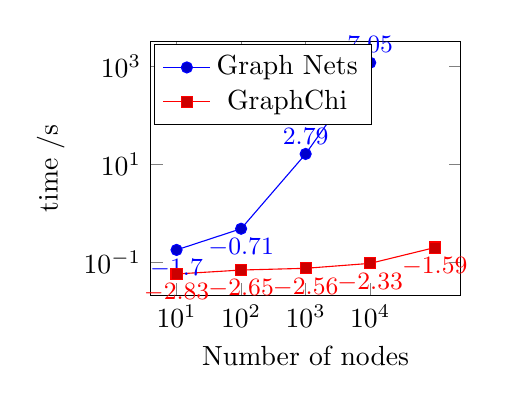
\begin{tikzpicture}
% CCl axis
\begin{axis}[
  %ybar,
  ylabel={time /s},
  ymode=log,
  xlabel=Number of nodes,
  symbolic x coords={$10^1$, $10^2$, $10^3$, $10^4$, $10^5$},
  xtick=data,
  nodes near coords,
  nodes near coords align={vertical}
]
\addplot coordinates {
($10^1$,0.182)
($10^2$,0.490)
($10^3$,16.224)
($10^4$,1157.622)
($10^5$,inf)
};
\addplot coordinates {
($10^1$,0.059)
($10^2$,0.071)
($10^3$,0.077)
($10^4$,0.097)
($10^5$,0.203)
};
    \legend{Graph Nets, GraphChi}
\end{axis}
\end{tikzpicture}
  \caption{CC}
\end{subfigure}%
\begin{subfigure}{.3\textwidth}
  \centering
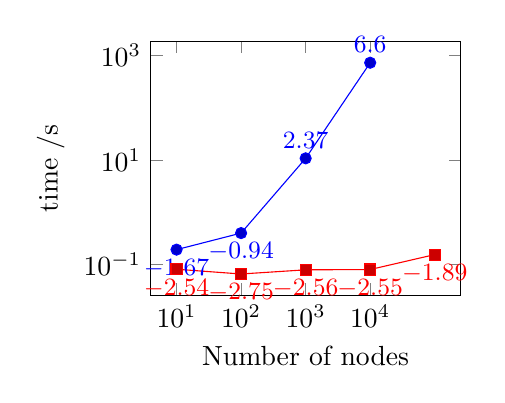
\begin{tikzpicture}
% SSSPl axis
\begin{axis}[
  %ybar,
  ylabel={time /s},
  ymode=log,
  xlabel=Number of nodes,
  symbolic x coords={$10^1$, $10^2$, $10^3$, $10^4$, $10^5$},
  xtick=data,
  nodes near coords,
  nodes near coords align={vertical}
]
\addplot coordinates {
($10^1$,0.188)
($10^2$,0.391)
($10^3$,10.678)
($10^4$,733.891)
($10^5$,inf)
};
\addplot coordinates {
($10^1$,0.079)
($10^2$,0.064)
($10^3$,0.077)
($10^4$,0.078)
($10^5$,0.151)
};
    \legend{}
\end{axis}
\end{tikzpicture}
  \caption{SSSP}
\end{subfigure}
\begin{subfigure}{.3\textwidth}
  \centering
  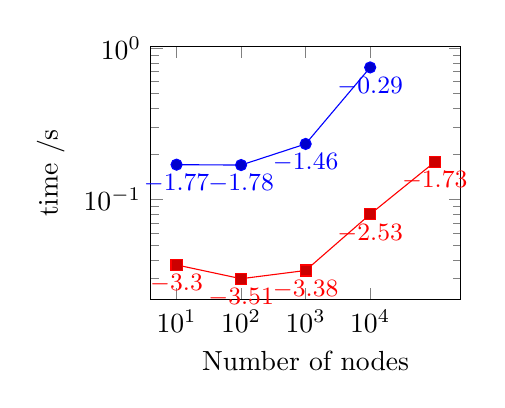
\begin{tikzpicture}
% PRl axis
\begin{axis}[
  %ybar,
  ylabel={time /s},
  ymode=log,
  xlabel=Number of nodes,
  symbolic x coords={$10^1$, $10^2$, $10^3$, $10^4$, $10^5$},
  xtick=data,
  nodes near coords,
  nodes near coords align={vertical}
]
\addplot coordinates {
($10^1$,0.170)
($10^2$,0.169)
($10^3$,0.233)
($10^4$,0.746)
($10^5$,inf)
};
\addplot coordinates {
($10^1$,0.037)
($10^2$,0.030)
($10^3$,0.034)
($10^4$,0.080)
($10^5$,0.177)
};
    \legend{}
\end{axis}
\end{tikzpicture}
  \caption{PR}
\end{subfigure}
\caption{Algorithm execution times running on linear graphs.}
\label{fig:linear}
\end{figure*}

As linear graphs have quite different properties to the others tested we can see that the results for linear graphs were quite different. As before, GraphChi was always faster and Graph Nets ran out of memory earlier. However, the interesting difference is the very different scaling. We can see that for CC and SSSP the GraphChi implementations seem to scale quite slowly in execution time. However, the scaling for Graph Nets is much higher. This is due to the asynchronicity of GraphChi as in every step there is no work to be done for most nodes in a linear graph for these algorithms but Graph Nets cannot take advantage of this. We can also see that this effect does not exist for PR. This is because the linear nature of the graph does not impact how much of it is updated in a step for PR.

\section{Discussion}

From the results we can see that Graph Nets is able to be used to execute graph algorithms. However, its performance does not come close to that of tools designed solely for this purpose. This is mainly down to how memory is used by TensorFlow and also the abstraction limits speed for many types of algorithms.

Beyond memory issues, the abstraction also makes it hard to implement algorithms with complicated message passing. This is because the messages from any edges must be reduced to a single numerical value before being read by a node. This means for more complicated algorithms a custom encoding would have to be used (which as it would extend outside pure tensor operations would dramatically slow execution).

So far we can see that Graph Nets is not useful for general purpose graph computation. However, we now examine what these results mean in the context of machine learning. The benefits from using this for machine learning are many. The main being that being part of the TensorFlow ecosystem we get most parts of training for free (which would require custom implementation in many other systems). Also, being part of the wider ecosystem it is very easy to add to existing systems and learn for current ML developers. However, as ML is used for larger graphs there may come scaling problems at which point a better framework for graph processing with the easy ability to learn parameters during training may need to be built from the ground up to take advantage of the aspects of graphs that can be parallelised. It turns out that some work has already been undertaken in this area such as in NGra\cite{better-graph-proc}.

\section{Conclusion}

In this paper we have assessed how the graph processing capacity of Graph Nets compares to a system designed specifically for this purpose (GraphChi). We have seen that Graph Nets in comparison is significantly slower and does not scale to large inputs. However, when taking into account the current priorities of the ML community the approach Graph Nets does make sense and performance is good enough. In spite of this, in the future other models may need to be explored for better scaling.

\subsection{Further work}

It seems at the current time that it is not sensible to build an easy to use API around Graph Nets for generic graph algorithm computing. However, this work does suggest that it would be interesting to examine the impact of embedding TensorFlow operations in a modern graph processing framework or building something new.

\bibliographystyle{ACM-Reference-Format}
\bibliography{refs}

\end{document}
\endinput
